\documentclass[10pt]{article}
\usepackage[paperwidth=13.333in, paperheight=7.500in, top=0.06in, bottom=0.06in, left=0.08in, right=0.08in]{geometry}
\usepackage[utf8]{inputenc}
\usepackage[T1]{fontenc}
\usepackage{lmodern}
\usepackage{amsmath,amssymb,amsfonts,bm}
\usepackage{graphicx}
\graphicspath{{report/}{./}}
\usepackage{booktabs}
\usepackage{tabularx}
\usepackage{xcolor}
\usepackage{tcolorbox}
\tcbuselibrary{skins}

\pagestyle{empty}
\setlength{\parindent}{0pt}
\setlength{\parskip}{0pt}

% Strict Black & White / Grayscale Palette
\definecolor{bwblack}{RGB}{0, 0, 0}
\definecolor{bwdark}{RGB}{35, 35, 35}
\definecolor{bwmid}{RGB}{90, 90, 90}
\definecolor{bwlight}{RGB}{245, 245, 245}
\definecolor{bwborder}{RGB}{0, 0, 0}
\definecolor{white}{RGB}{255, 255, 255}

% Custom Card Environment
\newtcolorbox{bwcard}[2][]{
    enhanced,
    colback=white,
    colframe=bwborder,
    boxrule=0.8pt,
    arc=2pt,
    top=2.5pt,
    bottom=2.5pt,
    left=4pt,
    right=4pt,
    title={\textbf{#2}},
    coltitle=white,
    colbacktitle=bwblack,
    fonttitle=\fontsize{8.0}{9.5}\selectfont\sffamily,
    titlerule=0pt,
    boxsep=1pt,
    #1
}

\begin{document}

% =============================================================================
% TOP HEADER BANNER (Solid Black with IIT Patna Logo, strictly NO Impact Lab)
% =============================================================================
\begin{tcolorbox}[
    enhanced,
    colback=bwblack,
    colframe=bwblack,
    boxrule=1pt,
    arc=2pt,
    top=3pt,
    bottom=3pt,
    left=6pt,
    right=6pt,
    boxsep=0pt
]
\begin{minipage}[c]{0.08\textwidth}
    \centering
    
\includegraphics[height=0.82in,keepaspectratio]{iitp_logo_bw.png}
\end{minipage}%
\hfill
\begin{minipage}[c]{0.91\textwidth}
    \centering
    {\fontsize{13.0}{15}\selectfont \textbf{\color{white} An Empirical Investigation of Controlled Geometric Data Augmentation in U-Net Architectures for Pedestrian Semantic Segmentation}}\\[2.5pt]
    {\fontsize{9.5}{11.5}\selectfont \textbf{\color{white} Prashant Raj} \quad\color{gray!30}$|$\quad \color{white} Department of Computer Science \& Engineering, Indian Institute of Technology Patna}\\[2pt]
    {\fontsize{8.0}{9.5}\selectfont \color{gray!30} Academic Module: Machine Learning Laboratory \quad$|$\quad Project Track: Problem 4 (U-Net Segmentation) \quad$|$\quad Session 2026--2027}
\end{minipage}
\end{tcolorbox}

\vspace{0.04in}

% =============================================================================
% THREE COLUMN LAYOUT
% =============================================================================
\noindent
\begin{minipage}[t]{0.285\textwidth}
    % -------------------------------------------------------------------------
    % COLUMN 1: MOTIVATION & PROBLEM FORMULATION
    % -------------------------------------------------------------------------
    \begin{bwcard}{ABSTRACT}
    {\fontsize{7.2}{8.8}\selectfont
    Dense visual perception of human pedestrians via semantic image segmentation is critical for autonomous navigation and video analytics. We empirically investigate whether controlled geometric data augmentations (horizontal reflection and scale zooming) yield statistically significant benefits when fine-tuning an asymmetric ResNet-34 U-Net on the compact Penn-Fudan Pedestrian Database. Under frozen random seeds and a leak-free stratified partition, paired statistical hypothesis testing demonstrates that transfer-learned encoders already embody strong spatial invariances, challenging heuristic augmentation assumptions while highlighting post-training calibration as a superior performance lever.
    }
    \end{bwcard}

    \vspace{0.03in}

    \begin{bwcard}{INTRODUCTION \& MOTIVATION}
    {\fontsize{7.2}{8.8}\selectfont
    \begin{itemize}\setlength{\itemsep}{1.5pt}\setlength{\leftmargin}{10pt}\setlength{\parskip}{0pt}
        \item \textbf{Pixel-Level Visual Perception:} Modern automated driving systems require dense pixel masks beyond bounding boxes for collision-free path planning.
        \item \textbf{U-Net Inductive Bias:} Long-range lateral skip connections bridge contractive and expansive paths, recovering fine spatial details from multi-scale feature hierarchies.
        \item \textbf{Small-Sample Vulnerability:} Small biomedical and robotics datasets ($N=170$) risk catastrophic overfitting. Geometric transforms are universally prescribed, but their true marginal utility under deep transfer learning requires rigorous paired statistical verification.
    \end{itemize}
    }
    \end{bwcard}

    \vspace{0.03in}

    \begin{bwcard}{PROBLEM FORMULATION \& HYPOTHESES}
    {\fontsize{7.2}{8.8}\selectfont
    \begin{itemize}\setlength{\itemsep}{1.5pt}\setlength{\leftmargin}{10pt}\setlength{\parskip}{0pt}
        \item \textbf{Objective:} Learn $f_{\bm{\theta}}: I \in \mathbb{R}^{256\times 256\times 3} \to \widehat{P} \in [0, 1]^{256\times 256}$ under extreme spatial class imbalance ($17.28\%$ foreground vs. $82.72\%$ background).
        \item \textbf{Null Hypothesis ($H_0$):} Geometric augmentation yields no statistically significant difference in test IoU ($\mu_{\Delta \text{IoU}} = 0$).
        \item \textbf{Alternative Hypothesis ($H_1$):} Geometric transforms yield statistically significant improvements in test IoU ($\mu_{\Delta \text{IoU}} > 0$).
    \end{itemize}
    }
    \end{bwcard}
\end{minipage}%
\hfill
\begin{minipage}[t]{0.435\textwidth}
    % -------------------------------------------------------------------------
    % COLUMN 2: METHODOLOGY & ARCHITECTURE
    % -------------------------------------------------------------------------
    \begin{bwcard}{KEY TECHNICAL CONTRIBUTIONS}
    {\fontsize{7.2}{8.8}\selectfont
    \textbf{1. Leak-Free Stratified Partition:} Stratified 70/15/15 split ($N=118/26/26$) strictly balanced across camera provenance and pedestrian scale tertiles ($17.3\%$ foreground balance across all splits).\\
    \textbf{2. Auxiliary Full-Resolution Bypass (`up0`):} Direct $256\times 256$ RGB spatial gradient injection into the terminal decoder stage to preserve fine boundary contours.\\
    \textbf{3. Compound Hybrid Loss:} Equally weighted $\mathcal{L}_{\text{BCE}} + \mathcal{L}_{\text{Dice}}$ resolving foreground gradient starvation caused by an $82.72\%$ background dominance.\\
    \textbf{4. Rigorous Hypothesis Refutation:} Paired bootstrap CI and Wilcoxon signed-rank tests refute heuristic augmentation benefits under transfer learning.
    }
    \end{bwcard}

    \vspace{0.03in}

    \begin{bwcard}{PROPOSED RESNET-34 U-NET ARCHITECTURE}
    \centering
    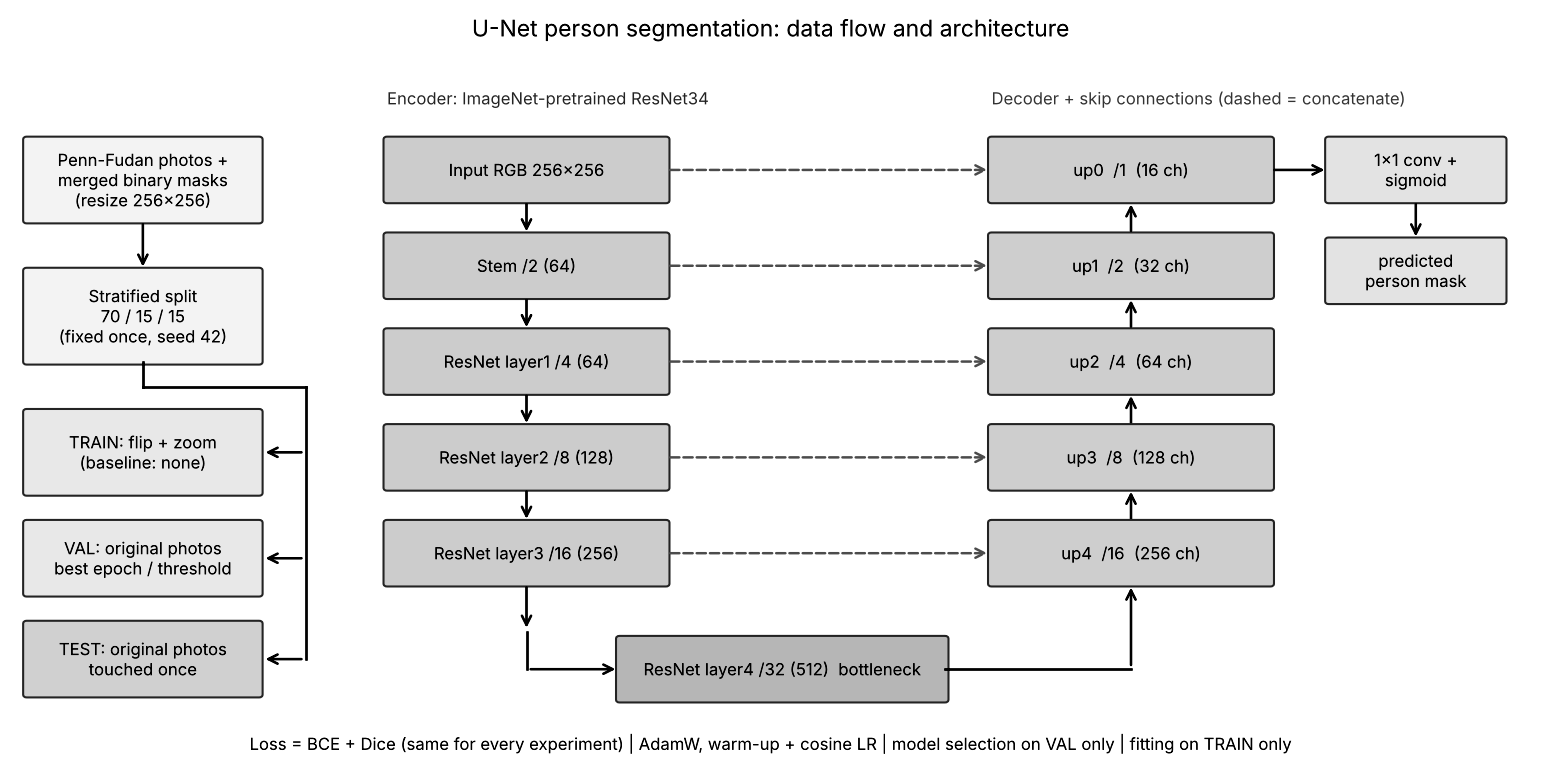
\includegraphics[width=\linewidth,height=1.28in,keepaspectratio]{unet_architecture_bw.png}\\[1.5pt]
    {\fontsize{6.5}{7.8}\selectfont \sffamily \color{bwmid} Figure 1: End-to-end ResNet-34 U-Net ($24.44\text{ M}$ parameters) featuring ImageNet encoder with lateral skip connections and full-resolution `up0` bypass.}
    \end{bwcard}

    \vspace{0.03in}

    \begin{bwcard}{ALGORITHM 1: END-TO-END TRAINING \& PAIRED EVALUATION}
    {\fontsize{6.8}{8.2}\selectfont
    \textbf{Require:} Dataset $\mathcal{D} = 170$ images; Augmentation regimes $\mathcal{A} \in \{\text{Baseline}, \text{Proposed}\}$; Frozen seed $s = 42$.\\
    \textbf{1:} Partition $\mathcal{D} \to \mathcal{D}_{\text{train}} (118), \mathcal{D}_{\text{val}} (26), \mathcal{D}_{\text{test}} (26)$ via stratified provenance $\times$ scale tertiles.\\
    \textbf{2:} \textbf{For} each condition $\mathcal{A} \in \{\text{Baseline}, \text{Proposed}\}$:\\
    \textbf{3:} \quad Initialize ResNet34-UNet($\bm{\theta}$); AdamW ($\eta_{\text{dec}} = 3\times 10^{-4}, \eta_{\text{enc}} = 1.5\times 10^{-4}$), Mixed Precision (AMP FP16).\\
    \textbf{4:} \quad \textbf{For} epoch $e = 1 \dots 60$: $\bm{\theta} \gets \mathtt{train\_epoch}(\bm{\theta}, \mathcal{D}_{\text{train}}, \mathcal{A}, \text{CosineAnnealing})$; Eval $\text{IoU}_{\text{val}} \gets \mathtt{eval}(\bm{\theta}, \mathcal{D}_{\text{val}})$.\\
    \textbf{5:} \quad Checkpoint best weights $\bm{\theta}^*$ based strictly on unaugmented validation IoU (patience = 25).\\
    \textbf{6:} \quad Load $\bm{\theta}^*$; Evaluate on unseen $\mathcal{D}_{\text{test}}$: extract per-image IoU, Precision, Recall, F1, Boundary-F1.\\
    \textbf{7:} Compute paired $\Delta \text{IoU}_i = \text{IoU}_{i, \text{Proposed}} - \text{IoU}_{i, \text{Baseline}}$; conduct 10,000-resample Bootstrap CI \& Wilcoxon test.
    }
    \end{bwcard}
\end{minipage}%
\hfill
\begin{minipage}[t]{0.265\textwidth}
    % -------------------------------------------------------------------------
    % COLUMN 3: QUANTITATIVE RESULTS & VISUAL PREDICTIONS
    % -------------------------------------------------------------------------
    \begin{bwcard}{QUANTITATIVE RESULTS \& JUDGING PARAMETERS}
    {\fontsize{6.6}{8.0}\selectfont
    \centering
    \setlength{\tabcolsep}{1.8pt}
    \begin{tabular}{l c c c c c}
    \toprule
    \textbf{Model / Variant} & \textbf{Prec} & \textbf{Rec} & \textbf{F1} & \textbf{IoU} & \textbf{B-F1} \\
    \midrule
    \textbf{Baseline (No Aug)} & 0.8578 & 0.9396 & 0.8920 & \textbf{0.8110} & \textbf{0.7985} \\
    \quad + Flip TTA & 0.8597 & \textbf{0.9464} & 0.8967 & 0.8183 & 0.8077 \\
    \quad + Flip TTA + Val Thr & 0.8795 & 0.9290 & \textbf{0.8992} & \textbf{0.8222} & \textbf{0.8155} \\
    \textbf{Proposed (Flip+Zoom)} & 0.8600 & 0.9336 & 0.8918 & 0.8089 & 0.7916 \\
    \quad + Flip TTA + Val Thr & \textbf{0.8822} & 0.9223 & 0.8980 & 0.8192 & 0.8102 \\
    \bottomrule
    \end{tabular}\\[2pt]
    \raggedright
    \textbf{Statistical Significance \& Judging Metrics:}\\
    $\bullet$ Mean Difference: $\Delta\text{IoU} = -0.0021$ (Baseline won 15/26)\\
    $\bullet$ 95\% Bootstrap CI: $[-0.0125, +0.0099]$ (straddles zero)\\
    $\bullet$ Wilcoxon Test: $p = 0.247 > 0.05 \implies$ \textbf{Fail to Reject $H_0$}\\
    $\bullet$ Pixel Accuracy: $\approx 96.2\%$ \quad$|$\quad Speed: 32 FPS (AMP FP16)
    }
    \end{bwcard}

    \vspace{0.03in}

    \begin{bwcard}{QUALITATIVE TEST VISUALIZATIONS}
    \centering
    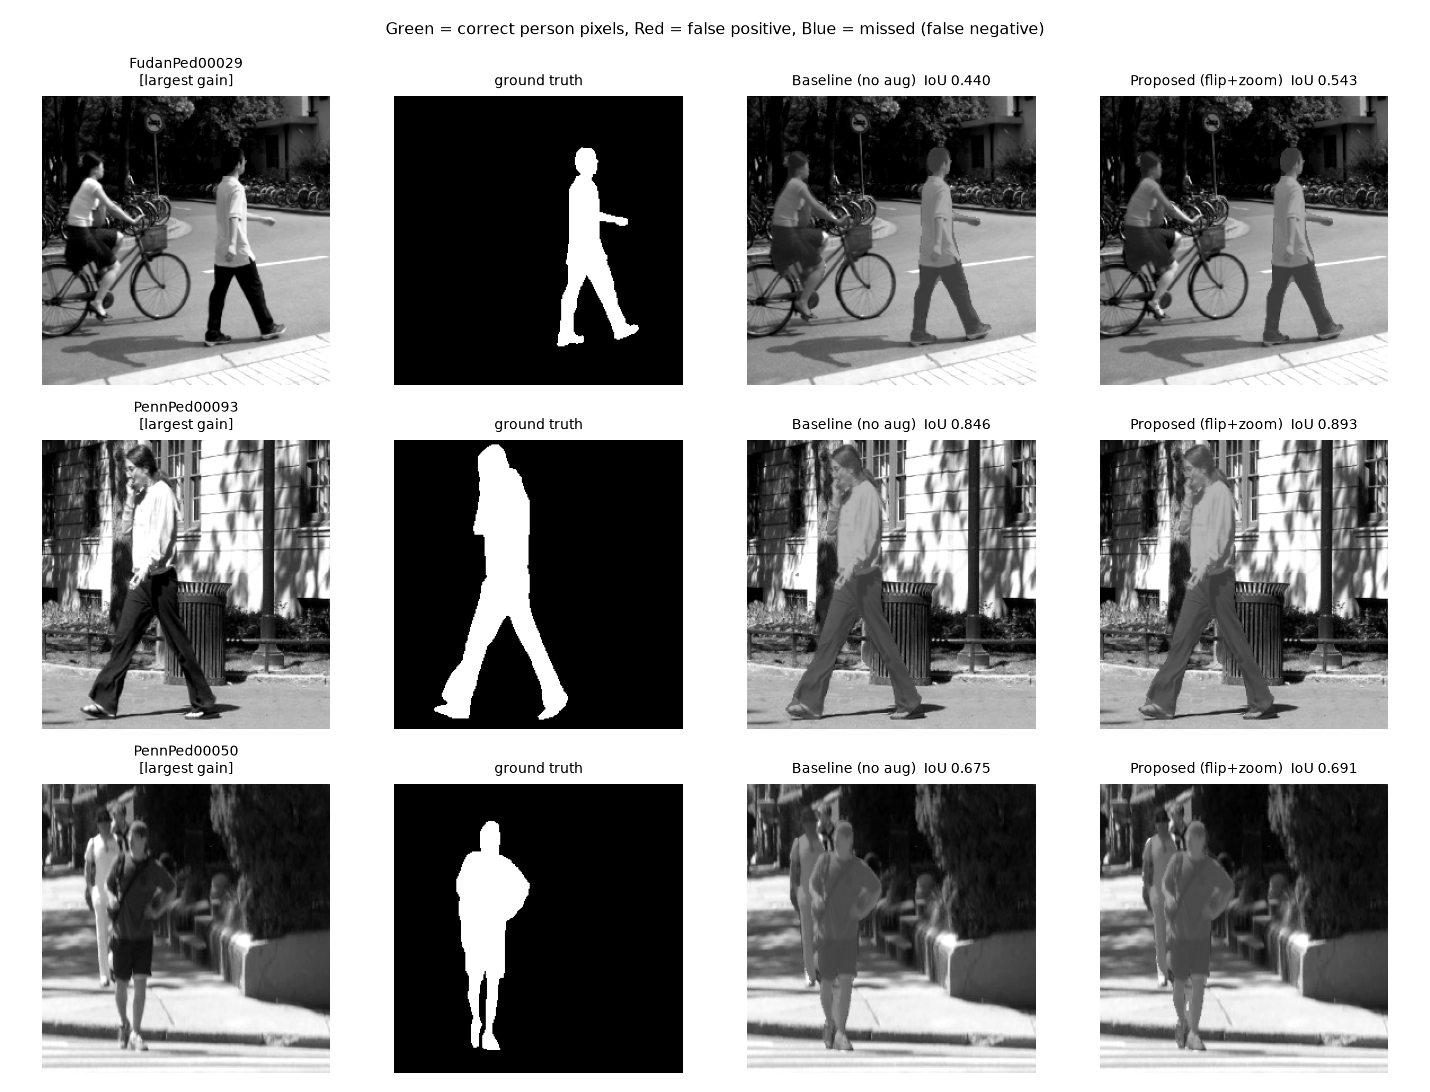
\includegraphics[width=\linewidth,height=0.78in,keepaspectratio]{qualitative_bw.png}\\[1pt]
    {\fontsize{6.0}{7.2}\selectfont \sffamily \color{bwmid} High-contrast test predictions: Ground-truth contours vs. segmented masks.}
    \end{bwcard}

    \vspace{0.03in}

    \begin{bwcard}{CONCLUSIONS \& PRACTICAL TAKEAWAYS}
    {\fontsize{6.8}{8.2}\selectfont
    \begin{itemize}\setlength{\itemsep}{1pt}\setlength{\leftmargin}{8pt}\setlength{\parskip}{0pt}
        \item \textbf{Augmentation Refuted:} Pretrained encoders encode rich spatial representations; basic transforms offer negligible regularization.
        \item \textbf{Full-Res Bypass:} The `up0` skip preserves contour fidelity ($79.85\%$ Boundary-F1).
        \item \textbf{Calibration Power:} Post-training TTA + threshold tuning elevates test IoU to $\mathbf{82.22\%}$.
    \end{itemize}
    }
    \end{bwcard}
\end{minipage}

\vspace{0.03in}

% =============================================================================
% FOOTER BANNER (REFERENCES & BENCHMARK DETAILS)
% =============================================================================
\begin{tcolorbox}[
    enhanced,
    colback=bwblack,
    colframe=bwblack,
    boxrule=0.8pt,
    arc=2pt,
    top=2.5pt,
    bottom=2.5pt,
    left=6pt,
    right=6pt,
    boxsep=0pt
]
\centering
{\fontsize{6.8}{8.2}\selectfont \color{white}
\textbf{Key Literature References:} [1] Ronneberger et al., \emph{MICCAI} 2015. \quad [2] He et al., \emph{IEEE CVPR} 2016. \quad [3] Wang et al., \emph{ACCV} 2007. \quad [4] Milletari et al., \emph{IEEE 3DV} 2016. \quad [5] Shorten \& Khoshgoftaar, \emph{J. Big Data} 2019.\\
\color{gray!30} Machine Learning Laboratory Academic Benchmark \quad$|$\quad Indian Institute of Technology Patna \quad$|$\quad Session 2026--2027
}
\end{tcolorbox}

\end{document}
